\chapter{Advanced strategies for Privacy-Enhancing Machine Learning}

\section{Differential Privacy}

\section{Homomorphic Encryption}

\section{Generative Models}

In Privacy Enhancing Machine Learning, generative models are being used to capture joint distributions of data in order to obtain synthetic samples without using real data. This can be used effectively to initialize deep learning models, perform data analysis, or apply it in competitions where models are initially validated using synthetic data and later tested (privately) with the original data.\\
The approach of this section will be to test the feasibility of using generative adversarial networks to extract data features and approximate their distribution. This is not done to train discriminative models with synthetic data, but rather to use synthetic data for tuning and designing models, thus enabling remote training (the model is trained locally where the data reside) without needing access to the original data, following the philosophy of Federated Learning (see section \ref{ch:Federated_Learning}). Comparing and evaluating the design of a Federated Learning model is beyond the scope of this work; instead, the distributions of the original datasets and synthetic datasets will be compared and evaluated.\\
In summary, two datasets will be used to test the feasibility of using generated data to facilitate model training in a Federated Learning environment, without necessarily using this data in the final model training. The aim is to approximate the distribution of the original dataset (a very challenging task). This could be done in conjunction with other techniques such as data anonymization, but this work will focus solely on generative models, particularly GANs. To assess the quality of synthetic data, scatter plots, histograms, and metrics measuring similarity in marginal distributions will be used.\\
The GAN (Generative Adversarial Network) architecture was originally proposed in \cite{goodfellow2014}. Since then, there have been numerous variations and improvements, primarily focused on image generation. Although other generative models exist, such as diffusion models, the GAN architecture remains employed and studied. In its original definition, the architecture consists of two models: a generative model $G$ that approximates the data distribution, and a discriminator model $D$ that estimates the probability that a sample is real or synthetic (generated by $G$). Both $G$ and $D$ are MLP (Multi-Layer Perceptron) architectures; in the case of $G$, the output dimension must match that of the real data. The main idea is that during training, these two models compete: $G$ seeks to learn to generate realistic data that can deceive $D$, while $D$ aims to correctly distinguish between real and generated samples from $G$. The input vector for $G$ consists of random noise, for example, $z \sim N(\mathbf{0}, \sigma \mathbf{I})$; denoted as $G = G(z) = G(z; \theta_g)$, where $\theta_g$ represents the network weights. The discriminator takes as input a real or synthetic data vector $x$, denoted interchangeably as $D = D(x) = D(x; \theta_d)$. The (simplified) training process is as follows:\\
First, the weights of $G$ and $D$ are initialized randomly. During each epoch, real data ${x_1,...,x_m}$ and random noise ${z_1,...,z_m}$ are sampled, where $x_i$ and $z_i$ have the same dimensions, for example, $x_i, z_i \in \mathbb{R}^p, \quad p \in \mathbb{N}$. In the case of tabular data, it can occur, for instance, $x_i, z_i \in \mathbb{R}^p \times \mathbb{Z}^k, \quad p,k \in \mathbb{N}$, if the table consists of $p$ columns of real data and $k$ columns of integer data. It can also occur that the data are categorical: if the i-th column is categorical, the i-th component of the vector $x$ and $z$ will take values in a finite set $\Omega$ that can be numerically encoded. This will affect the exact definition of the initial (a priori) distribution of $z$.

Next, the batch of synthetic samples ${G(z_1),...,G(z_m)}$ is computed. Now $D$ receives both the batch of real data ${x_1,...,x_m}$ and the batch of synthetic data ${G(z_1),...,G(z_m)}$ and must distinguish between them. Therefore, $D$ is a discriminative (supervised) binary classification model; it classifies as 1 the data it confidently predicts as real and as 0 the synthetic data ($D$ outputs a probability between 0 and 1). Based on this classification, the discriminator's loss function is calculated, and $D$'s weights are adjusted to \textbf{minimize} this loss.

Next, another batch of synthetic data ${G'(z_1),...,G'(z_m)}$ is generated, and $G$'s loss is computed as it tries to deceive the discriminator (which has already been updated). $G$'s weights are updated to \textbf{maximize} this loss. This process is repeated iteratively until a stopping criterion is met, such as a maximum number of epochs.

Therefore, this involves the following min-max game:
\begin{equation}
\min_G \hspace{0.3 em} \max_D V(G,D) = E_{x \sim \rho_{\text{data}}(x)}[\log D(x)] + E_{z \sim \rho_z(z)}[\log(1 - D(G(z)))]
\label{eq:funcion_objetivo_GAN}
\end{equation}

The intuitive idea behind this formula is as follows: the ultimate goal of the architecture is for $\rho_z$ to converge to $\rho_{\text{data}}$, meaning that $G$ should approximate the theoretical data distribution perfectly (although $\rho_{\text{data}}$ is unknown and we only have a finite sample of data). To achieve this, we use $D$: if there were a perfect discriminator that could distinguish between real and synthetic data, we could use it to update the weights of $G$ and improve the generative model. The approach is to train both models simultaneously with the aim of achieving perfect models: where $D$ correctly classifies the data, maximizing the probability of classifying samples drawn from $\rho_{\text{data}}$ as real, and minimizing the probability of classifying samples generated by $G$ as real. This is expressed as:
\begin{equation*}
\max_D V(G,D) = E_{x \sim \rho_{\text{data}}(x)}[\log D(x)] + E_{z \sim \rho_z(z)}[\log(1 - D(G(z)))]
\end{equation*}

At the same time, given a discriminator $D$, we want $G$ to maximize the probability that $D$ classifies samples drawn from $\rho_z$ as real. This can be formulated as:
\begin{equation*}
\max_G V(G,D) = E_{z \sim \rho_z}[\log D(G(z))] \Leftrightarrow \min_G V(G,D) = E_{z \sim \rho_z} [\log(1 - D(G(z)))]
\end{equation*}

These two formulations lead us to (\ref{eq:funcion_objetivo_GAN}).\\
\textbf{Note:} In implementations, care is taken to ensure that the probability returned by $D$ is not exactly 0 or 1 to avoid $\log$ from approaching 0.\\

Taking this into account, we can now understand the expressions given in the original paper \cite{goodfellow2014} for updating the model weights. Let's start with $D$, which receives batches of real data ${x_1,...,x_m}$ and synthetic data ${G(z_1),...,G(z_m)}$. Stochastic gradient ascent is applied as follows:

\begin{equation*}
\theta_{d}' = \theta_d + \eta \frac{\partial }{\partial \theta_d} \left[ \frac{1}{m} \sum_{i=1}^m \left( \log D(x_i) + \log (1 - D(G(z_i))) \right) \right]
\end{equation*}

\textbf{Note:} We take the mean of individual losses, which represents the empirical risk: an estimation of the theoretical risk since we do not know the theoretical data distribution. I emphasize the $+$ sign, as our goal is to maximize.

For $G$, the weights are updated using stochastic gradient descent as follows:

\begin{equation*}
\theta_{g}' = \theta_g - \eta \frac{\partial}{\partial \theta_g} \left[ \frac{1}{m} \sum_{i=1}^m \log(1 - D(G(z_i))) \right]
\end{equation*}

\textbf{Note:} This is a simplified version of stochastic gradient methods. The original paper mentions using a variant with momentum (see section \ref{sec:optimizer}). There are many variations with different hyperparameters and features. A deliberately simplified terminology has been maintained.

Since both $G$ and $D$ are MLPs, gradients can be efficiently computed using the backpropagation algorithm.

For tabular datasets, certain particularities must be addressed (\cite*{xu2019}). In particular, we will use a variant of the original GAN: the Conditional GAN. We will consider features (columns) of both continuous and discrete data. The generator model must differentiate between the two; in the final layer, a $softmax$ activation function will be used for the discrete case and $tanh$ for the continuous case.

\begin{align*}
tanh(x) &= \frac{e^x - e^{-x}}{e^x + e^{-x}} \quad x \in \mathbb{R} \\
softmax (\mathbf{x})_j &= \frac{e^{x_j}}{\sum{i=1}^n e^{x_i}} \quad j=1,...,n \quad \mathbf{x} \in \mathbb{R}^n
\end{align*}

In a conditional GAN, both the generator and the discriminator also receive additional information, which can be in the form of class labels, specific features, or any other relevant information for the problem at hand. This additional information is provided as a condition for the generation of synthetic samples and the evaluation of their authenticity.

Introducing conditional information into a GAN allows for more specific control over the generation process. For example, in the case of image generation conditioned on certain class labels, a conditional GAN can generate images of a specific type, such as "cats" or "dogs," according to the label provided as the condition.

In the context of CTGAN (Conditional Tabular Generative Adversarial Networks), this additional information can be any relevant feature or set of features present in the original data. For example, if working with a tabular dataset containing information about bank customers, the additional information could include the customer's gender, age, account type, credit history, etc.

During the training process of the CTGAN, both the generator and the discriminator receive this additional information as a condition for the generation and evaluation of synthetic data. This means that the generator learns to generate synthetic samples that are not only statistically similar to the original data but also conditioned on specific values of the provided features.

For example, if one wants to generate synthetic data of bank customers with a certain age range and gender, this information can be provided as a condition to the CTGAN during the generation process. As a result, the CTGAN will be able to generate synthetic samples that follow the distributions of the conditioned features, which can be useful in various applications, such as generating balanced training data, preserving privacy, or conducting sensitive testing. In summary, CTGAN applies the principles of conditional GANs to the specific context of tabular data synthesis.

When working with tabular data instead of images, several aspects must be considered, such as continuous variables not typically following a normal distribution; in fact, they may follow a multimodal distribution (having more than one peak of maximum density). Additionally, there can be issues of imbalanced features (for example, in the case of banking data, a binary variable determining default status is often very imbalanced, as most customers are not defaulters).

To numerically evaluate the synthetic datasets, the KSComplement and TVComplement metrics from the \textit{SDMetrics} library will be used. The KSComplement metric calculates the similarity (of the marginal distribution) between two columns, one real and one synthetic. It uses the Kolmogorov-Smirnov statistic, which measures the maximum difference between two cumulative probability distributions, yielding a value between 0 and 1. KSComplement returns $1-KS$, meaning the closer to 1, the more similar the distributions. This metric will be used for continuous variables. For categorical variables, the TVComplement metric from the same library will be used, which also measures the similarity between two marginal distributions. It calculates the frequentist probability of each class and sums the absolute differences for each class. The metric returns $1-\text{result}$, so the closer the value is to 1, the better the distributions match.

\textbf{Results:}

For the implementation, the CTGAN library in Python has been used. This library addresses the problem of non-Gaussian and multimodal data through variational Gaussian mixture models to estimate complex distributions. Explaining Gaussian mixtures is beyond the scope of this work, but \cite*{bishop2006} has been used as a reference for this type of model.

A total of 2 datasets have been used to check the performance of CTGAN. The first consists of a dataset generated by myself, composed of two columns $x$ and $y$ that follow a normal distribution $N(\mu, \Sigma)$, where $\mu = \begin{pmatrix}
0 \
0
\end{pmatrix}$ and $\Sigma = \begin{pmatrix}
1 & 0.5 \
0.5 & 1
\end{pmatrix}$, meaning they are positively correlated variables. The third column is a categorical feature with 5 classes encoded with numbers from 0 to 4. These classes have been generated using the probability vector $p=(0.3, 0.2, 0.4, 0.07, 0.03)$. A thousand samples of this dataset have been generated, and CTGAN was trained for 3000 epochs. This is a somewhat arbitrary stopping criterion after observing the objective function graphs, as the loss curves of $G$ and $D$ oscillate and do not reach Nash equilibrium. Theoretically, the optimum is reached when $D = 1/2$, that is, when it is unable to differentiate between real and synthetic data and determines this randomly. The goal of this work is not to train the best possible model but to study its feasibility according to the privacy objectives set.

A thousand rows of $\rho_z$ were sampled:


\begin{figure}[htbp]
    \centering
    \begin{minipage}[b]{0.4\textwidth}
      \centering
      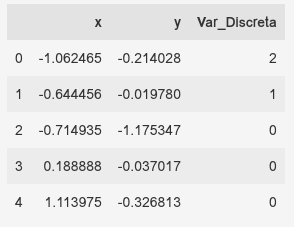
\includegraphics[width=0.6\textwidth]{figures/4-Advanced_Strategies/Ejemplo_Dataset_1_Real.png}
      \caption{Real samples}
    \end{minipage}
    \hfill
    \begin{minipage}[b]{0.4\textwidth}
      \centering
      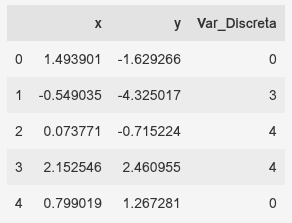
\includegraphics[width=0.6\textwidth]{figures/4-Advanced_Strategies/Ejemplo_Dataset_1_Sintetico.png}
      \caption{Synthetic samples}
    \end{minipage}
\end{figure}

\begin{figure}[H]
    \centering
    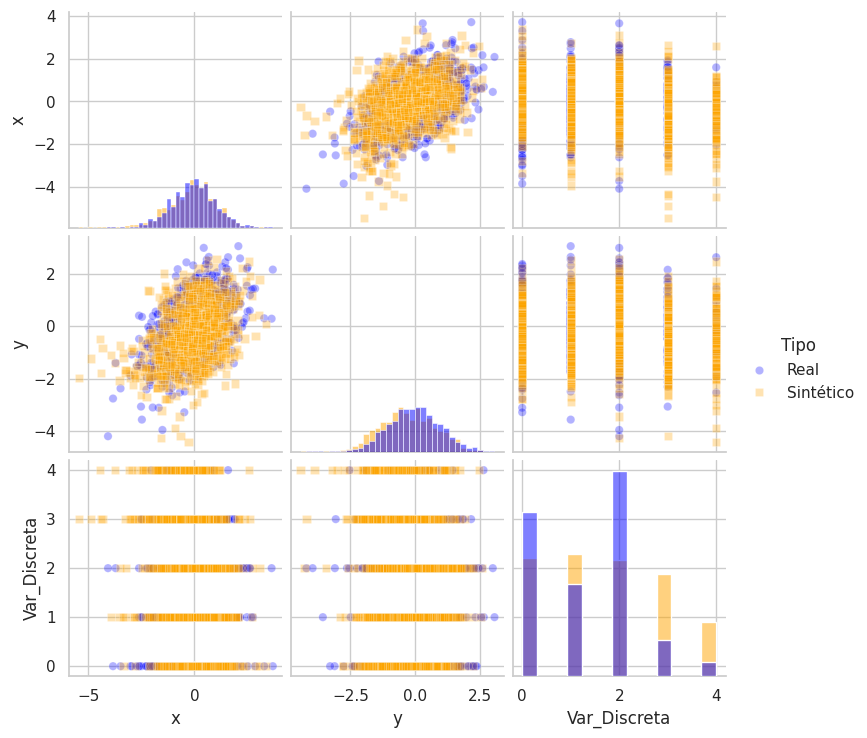
\includegraphics[scale=.35]{figures/4-Advanced_Strategies/pairplot_Dataset1.png}
    \caption{Scatter plot and histogram.}
\end{figure}

\begin{itemize}
    \item KS-Complement x: 0.94
    \item KS-Complement y: 0.887
    \item TV-Complement discrete variable: 0.773
\end{itemize}

For the second test, the Iris dataset has been used, which contains 4 continuous features and 1 categorical feature (encoded as a discrete variable from a finite set). This dataset contains few samples (150 in total), so the estimation of the distribution may be affected by the small amount of real data. It was trained for 1500 epochs in a few seconds. The 'species' variable was encoded as \{ 'setosa': 0, 'versicolor': 1, 'virginica': 2 \}. After training, 150 data points were sampled from the generated distribution:\\

\begin{figure}[htbp]
    \centering
    \begin{minipage}[b]{0.4\textwidth}
      \centering
      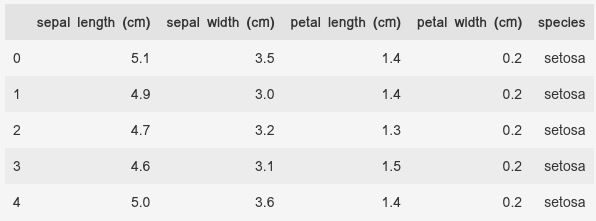
\includegraphics[width=0.6\textwidth]{figures/4-Advanced_Strategies/Ejemplo_Dataset_2_Real.png}
      \caption{Real samples}
    \end{minipage}
    \hfill
    \begin{minipage}[b]{0.4\textwidth}
      \centering
      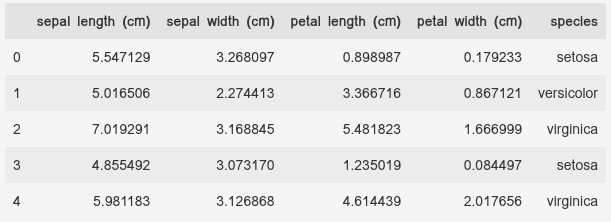
\includegraphics[width=0.6\textwidth]{figures/4-Advanced_Strategies/Ejemplo_Dataset_2_Sintetico.png}
      \caption{Synthetic samples}
    \end{minipage}
\end{figure}

\begin{figure}[H]
    \centering
    \includegraphics*[scale=.3]{figures/4-Advanced_Strategies/pairplot-Dataset2.png}
    \caption{Scatter plot and histogram.}
\end{figure}

\begin{itemize}
    \item KS-Complement sepal length (cm): 0.91
    \item KS-Complement sepal width (cm): 0.85
    \item KS-Complement petal length (cm): 0.89
    \item KS-Complement petal width (cm): 0.8
    \item TV-Complement species: 0.96
\end{itemize}

We observe that in both datasets, a high marginal similarity of the columns has been achieved (close to 1). The scatter plots show that the model has relatively well captured the correlations between variables, and the histograms between real and synthetic data are quite similar. However, good performance in these datasets does not necessarily imply it is a good model. It is currently known that there are models that better capture the distribution of tabular data, although the use of GANs can still be useful in this task. Available resources, such as computing power or the amount of data, will guide the choice between different methods.\\
The generation of synthetic tabular data using GANs can be an additional tool in the set of technologies aiming to train models with sensitive data while safeguarding privacy. The quality of synthetic data depends on many factors: the original dataset size, imbalanced classes, etc. However, these networks seem to approximate the distribution of the original data, though not perfectly. Approximating the joint distribution is a very complex problem to solve, and in this work, only very simple datasets have been used, and even with these datasets, it has not been possible to perfectly approximate the original distribution.

This is why, although it is a promising technique, I do not believe it is appropriate to use it for conducting scientific studies or training models solely using synthetic data. Nonetheless, they do fulfill the intended function: serving as a guide for adjusting models in a Federated Learning environment without needing to share the original data. With synthetic data, the different entities that hold the data can share these synthetic data to help researchers understand, albeit approximately, the type of data they need to work with.

For this purpose, I believe that data generation can be helpful. It should be studied to what extent generative models can resist attacks aimed at extracting information about the original data (\cite*{sun2023}), although this is beyond the scope of this work.
